\documentclass{vldb}
\usepackage{graphicx}
\usepackage{caption}
\usepackage{subcaption}
%\usepackage{balance} 
\usepackage{epstopdf}
\usepackage{pbox}
\let\proof\relax
\let\endproof\relax
\usepackage{algorithm, algpseudocode, amsmath,amsthm,amssymb}

\graphicspath{ {./charts/}, {./exp/} }
\epstopdfsetup{outdir=./charts/}
\newcommand{\reminder}[1]{ {\mbox{$<==$}} [[[ { \bf #1 } ]]] {\mbox{$==>$}}}
\newtheorem{definition}{Definition}
\newtheorem{theorem}{Theorem}
\newtheorem{example}{Example}
\DeclareMathOperator*{\argmin}{argmin}
\DeclareMathOperator*{\argmax}{argmax}
\newcommand*{\argminl}{\argmin\limits}
\newcommand*{\argmaxl}{\argmax\limits}

\hyphenation{op-tical net-works semi-conduc-tor}

\begin{document}

% ****************** TITLE ****************************************

\title{A Parallel Platform for Mining General Co-Movement Patterns over Large-scale Trajectories}

% ****************** AUTHORS **************************************

% You need the command \numberofauthors to handle the 'placement
% and alignment' of the authors beneath the title.
%
% For aesthetic reasons, we recommend 'three authors at a time'
% i.e. three 'name/affiliation blocks' be placed beneath the title.
%
% NOTE: You are NOT restricted in how many 'rows' of
% "name/affiliations" may appear. We just ask that you restrict
% the number of 'columns' to three.
%
% Because of the available 'opening page real-estate'
% we ask you to refrain from putting more than six authors
% (two rows with three columns) beneath the article title.
% More than six makes the first-page appear very cluttered indeed.
%
% Use the \alignauthor commands to handle the names
% and affiliations for an 'aesthetic maximum' of six authors.
% Add names, affiliations, addresses for
% the seventh etc. author(s) as the argument for the
% \additionalauthors command.
% These 'additional authors' will be output/set for you
% without further effort on your part as the last section in
% the body of your article BEFORE References or any Appendices.

%\author{
%	\IEEEauthorblockN{
%		Qi Fan\IEEEauthorrefmark{1},
%		Yuchen Li\IEEEauthorrefmark{1},
%		Dongxiang Zhang\IEEEauthorrefmark{2} and
%		Kian-Lee Tan\IEEEauthorrefmark{1}\IEEEauthorrefmark{2}
%		}
%	\IEEEauthorblockA{
%		\IEEEauthorrefmark{1}NUS Graduate School for Integrative Sciences and Engineering,
%		National University of Singapore, Singapore\\
%		\{fan.qi, liyuchen\}@nus.edu.sg
%	}
%	\IEEEauthorblockA{
%		\IEEEauthorrefmark{2}School of Computing,
%		National University of Singapore, Singapore \\
%		\{zhangdo,tankl\}@comp.nus.edu.sg
%	}
%}

\maketitle

\begin{abstract}

\end{abstract}


\section{Introduction}
The prevalence of positioning devices has drastically boosted the scale of trajectory data collection. 
Instances include telemetry chips for animal herding histories, 
GPS devices for urban transportation and wearable devices for personal moving activities. 
These positional data are timestamped and can be viewed as trajectories. 
Data analysis on large-scale trajectories benefits a wide range of applications and services, including traffic planning~\cite{zheng2011urban}, animal analysis~\cite{li2010miningperiodic}, and social recommendations~\cite{bao2013survey}, just to name a few.% CITATIONS FOR THE ABOVE APPLICATIONS.

An important task of data analysis on trajectories is to discover co-moving objects. 
As its name suggests, a \emph{co-movement} pattern~\cite{li2013managing} consists 
of a group of objects that travel together for some duration, where the group is formed
by certain clustering methods. A pattern is prominent 
if the size of the group exceeds $M$ and the length of the duration exceeds $K$, where $M$ and $K$
are user specified parameters. Depends on further constraints on object clustering
and time duration, several specific patterns are proposed in the literature. 

Specifically, on the aspect of object clustering, \emph{flock}~\cite{gudmundsson2006flock} and \emph{group}~\cite{wang2006grouppattern} patterns require objects to be within a disk region.
In contrast, \emph{convoy}~\cite{jeung2008convoy}, \emph{swarm}~\cite{li2010swarm} and
\emph{platoon}~\cite{li2015platoon} patterns require objects to be densely connected. 
In terms of the constraints on time duration, \emph{flock}~\cite{gudmundsson2006flock} and \emph{convoy}~\cite{jeung2008convoy}
require the timestamps to be consecutive. \emph{Swarm}~\cite{li2010swarm}, on the
other hand, do not impose any restrictions. \emph{Group}~\cite{wang2006grouppattern} 
and \emph{platoon}~\cite{li2015platoon} introduce the parameter $L$ to control the minimum length of the local-consecutive
timestamps. 
The compare and contrast of these co-movement patterns are presented in Table~\ref{tbl:existing_co_patterns}.

%Specifically, a \emph{flock}~\cite{gudmundsson2006flock} requires the group to be within a disk region of
%the user specified size.  A \emph{convoy}~\cite{jeung2008convoy} requires a group to be densely connected. Both \emph{flock}
%and \emph{convoy} require a group to appear for at least $k$ consecutive times.  
%\emph{Group}~\cite{wang2006grouppattern} and 
%\emph{Swarm}~\cite{li2010swarm} patterns relax the consecutiveness constraint, where non-consecutive timestamps are allowed in a pattern duration. \emph{Group} pattern require objects in a group to be within a disk region, while \emph{swarm}require the objects in a group to be densely connected.
%Recently,
%\emph{platoon}~\cite{li2015platoon} pattern is proposed to impose a fine-grained control on the consecutiveness of the duration. In \emph{platoon}, the duration of a group needs to have the local-consecutive portion of size no less than the user-specified $L$.

\begin{table}
\centering
\begin{tabular}{|c|c|c|c|}
\hline 
Pattern & Clustering Method & Consecutiveness on Duration \\ 
\hline 
Flock~\cite{gudmundsson2004flock} & Disk region &  Consecutive \\ 
\hline 
Convoy~\cite{jeung2008convoy} & Density &   Consecutive \\ 
\hline 
Group~\cite{wang2006grouppattern} & Disk region &  Local consecutive $\geq L$ \\ 
\hline 
Swarm~\cite{li2010swarm} & Density  & No constraint \\ 
\hline 
Platoon~\cite{li2015platoon} & Density &  Local consecutive $\geq L$ \\ 
\hline 
\end{tabular} 
\caption{Existing Co-movement Patterns}
\label{tbl:existing_co_patterns}
\end{table}

%of densely connected objects that travel together for at least $k$ consecutive time. A \emph{swarm}~\cite{li2010swarm} relax the consecutiveness of \emph{convoy}.
% 
%To formally define the pattern, the temporal dimension of trajectories is descritized into snapshots, where each snapshot contains the geographical information of all moving objects. 
%Given a member size constraint $n$, a temporal constraint $k$, a \emph{co-movement} pattern finds a cluster of objects with at least size $n$ and close in spatial proximity for at least $k$ snapshots. 
%Recently, there have been several works extending the basic pattern to incorporate more advanced temporal constraints. For instance, Jeung et al. proposed \emph{convoy} pattern, which requires the snapshots to be consecutive; Li et al. proposed \emph{swarm} pattern, which relaxes the consecutiveness of snapshots and Li et al. proposed \emph{platoon} pattern which imposed a \emph{minimum local length} on the snapshots. 
%PLEASE BE MORE SPECIFIC FOR THE THREE PATTERNS. ALSO, ADD THE CITATIONS.


%We first provide a synthetic example to better illustrate these patterns in Figure~\ref{fig:related_work}, and the formal definitions are described in Section~\ref{sec:definition}.
We illustrate these co-movement patterns in Figure~\ref{fig:related_work} with an example of five trajectories.
First, the temporal domain is discretized into five snapshots. 
In each snapshot, the objects are clustered as shown in the dotted circle.
By setting the parameters $M=2, K=3$, we are able to discover \emph{convoy}, \emph{flock}, and \emph{swarm} patterns. 
It is notable that \emph{convoy} and \emph{flock} have the same result pattern, this is because both patterns share 
the same constraints on the time duration. 
\emph{Swarm} pattern results in a super set of \emph{convoy} and \emph{flock} patterns, as it 
does not require any consecutiveness on the time duration. By setting $L=2$, we find three \emph{group} patterns. 
If further set $M=2,K=3$, two \emph{platoon} patterns are found. It is observable that the pattern $\langle\{O_5,O_6\}\{1,4,5\} \rangle$ is a \emph{swarm} but is neither a \emph{platoon} nor a \emph{group} since one of its local consecutive duration (i.e. $\{1\}$) is less than $2$. However, $\langle\{O_5,O_6\}\{1,4,5\} \rangle$ can be reduced to $\langle\{O_5,O_6\}\{4,5\} \rangle$ which is a \emph{group} pattern because \emph{group} pattern only restricts the local consecutiveness but not the total size of a duration. 

% we achieve two \emph{platoon} patterns.
% 
%By setting $M=2$, the spatial clusters with at least $2$ objects are displayed with the same shape. Since \emph{Convoy} pattern requires the set of objects to be clustered for $k$ \emph{consecutive} snapshots, there results in only one such pattern ($\{o_3,o_4\}\{t_1,t_2,t_3\}$) when $k$ is set to $3$. \emph{Swarm} pattern relaxes the consecutiveness of duration, thus there are three patterns discovered. \emph{Platoon} pattern requires that each local consecutive duration needs to have at least certain length, which is indicated by an additional parameter $l$. When $l$ equals 2, there are two patterns discovered. Note that $\{o_6,o_7\}\{t_1,t_4,t_5\}$ is not included in the platoon pattern since $t_1$ is the local consecutive snapshot with duration 1, which is less than $l$. CAN WE SUPPORT THE GROUP AND FLOCK PATTERN? IF YES, WHY NOT PUT THEM IN THE FIGURE?
%
%FOR THE FIGURE: 1) ENLARGE THE FONT SIZE IN THE FIGURE 2) WHY THERE IS NO $o_5$. 3) WHY OBJECTS IN DIFFERENT COLORS AND SHAPES ARE NOT CLEAR. YOU CAN REMOVE COLOR. 4) PUT THE OBJECTS BELONGING TO THE SAME CLUSTER IN THE SAME LINE.

\begin{figure} [h]
\center
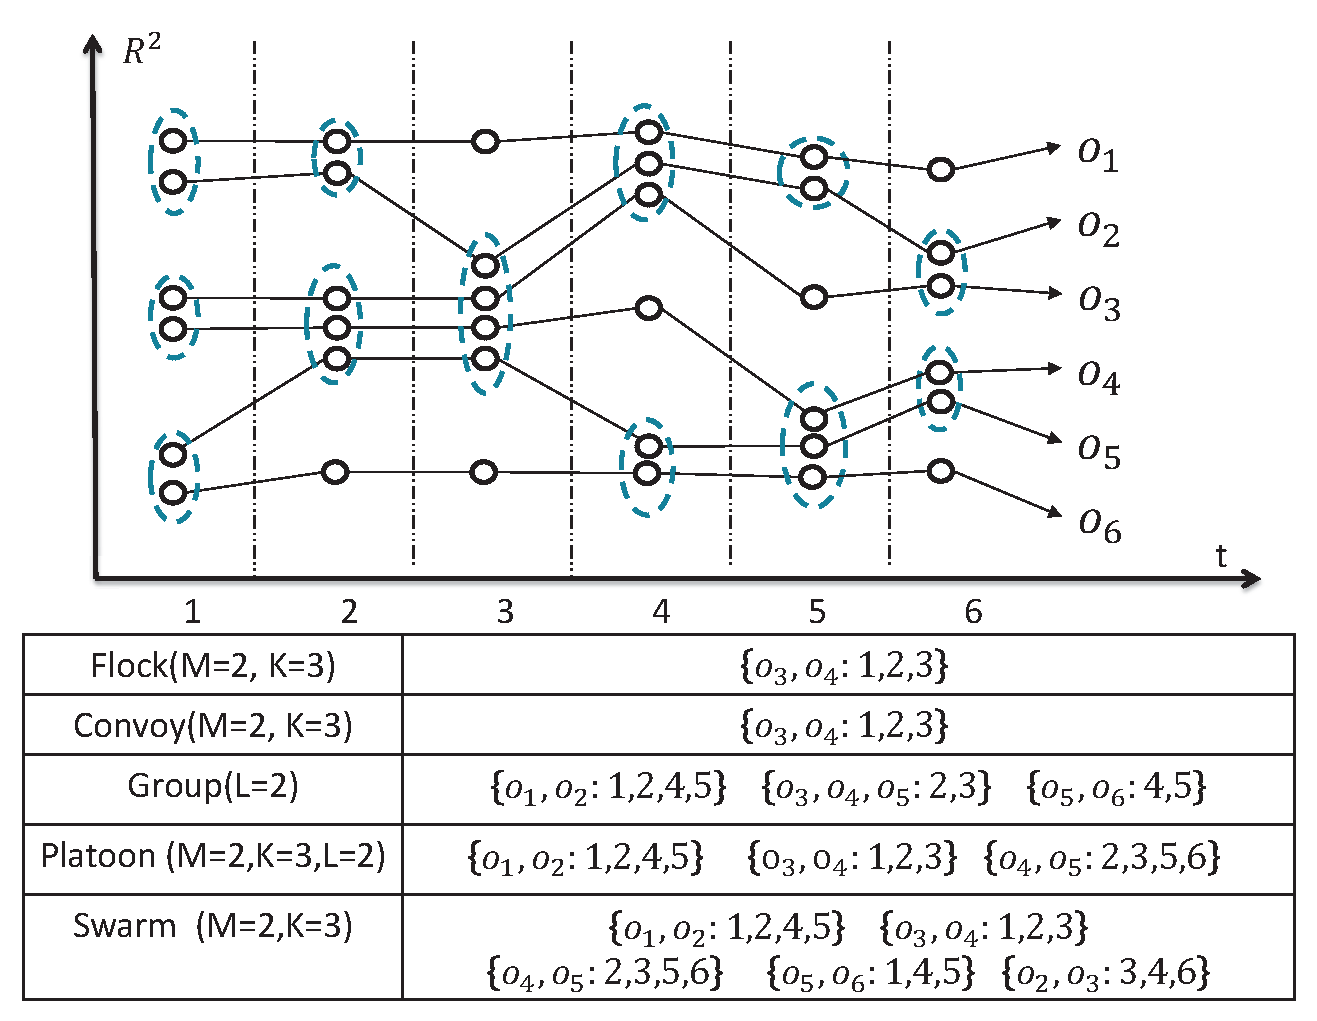
\includegraphics[width=0.5\textwidth]{related_work.eps}
\caption{Trajectories and Co-Movement Patterns}
\label{fig:related_work}
\end{figure}

%We notice that, \emph{platoon} pattern is more general than \emph{convoy} and \emph{swarm}. This is because by setting appropriate $l$, \emph{platoon} can be reduced to \emph{convoy} and \emph{swarm} respectively~\cite{li2015platoon}. However, we observe that \emph{platoon} pattern is to loose on the temporal domain thus may result in less significant patterns. For example in Figure~\ref{fig:platoon_weakpoint}.


%
%\begin{figure}[h]
%\center
%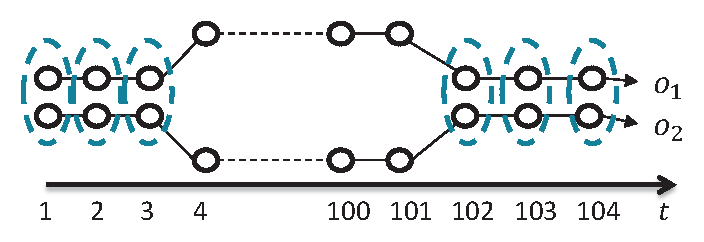
\includegraphics[width=0.5\textwidth]{platoon_weakpoint.eps}
%\caption{Miss-pattern in platoon}
%\label{fig:platoon_weakpoint}
%\end{figure}

%In platoon, a pattern for $n=2,k=4,l=2$ could be $\{o_1, o_2\}\{t_1,t_2,t_4,t_5,t_{100},t_{101}\}$. However, the snapshots $t_{100}$ and $t_{101}$ is too far away from previous snapshots. Such two snapshots are in less relation with previous snapshots and thus should be removed from the pattern. Based on this observation, we defined a \emph{generalized co-moving} pattern (as in Section~\ref{sec:definition}) to provide a more fine granular control of the pattern. In \emph{generalized co-moving} pattern, a parameter $g$ is introduce the control the \emph{maximum gap} allowed between consecutive snapshots. By so doing our generalized co-moving pattern is more expressive and can represent all the existing co-moving patterns.

%In step with the advances in localization technologies, the growth in the volume of trajectory data is rapid. Traditional single-machine methods face severe scalability problem in handling large trajectory data. For example, as reported in~\cite{li2015platoon}, a \emph{Swarm} pattern takes around 100 seconds to discover for 100k trajectories. With upto billions of trajectories in nowadays datasets, such approaches apparently become unfeasible. To tackle this challenge, we propose a  paralleled solution for discovering \emph{generalized co-moving} patterns. We then deploy our idea on the modern MapReduce platform. As our experiments show, our solution achieves well load-balance and can process billions of trajectories in XXX seconds. Several optimizations are also designed to boost our solution to be orders of magnitudes faster than baseline algorithms.

%In practice, it is cumbersome to design tailed solutions to different types of co-movement pattern discovery. 

%In reality, it is cumbersome to design tailed solutions to support 
%generality and scalability

%In this paper, our primary objectives are solving two 

As can be seen, there are various co-movement patterns requested by different applications and it is cumbersome to design a tailored solution for each type. Hence, there is an urgent demand for a general platform to support all these co-movement patterns. Another issue with existing methods is that they are built on top of centralized indexes that are not scalable. The maximum number of trajectories ever evaluated is up to hundreds of thousands of trajectories. In practice, it is rather common to collect millions of trajectories. We, for the first time, evaluate the pattern mining performance at the million scale and report the performance in Figure~\ref{}. The results show that their performance degrades dramatically as the dataset size scales up. None of them can handle millions of trajectories efficiently. 

Therefore, our primary contributions in this paper are to close these two gaps. First, we propose a general co-movement pattern definition to incorporate all the related variants in the existing literature. We observe that even though \emph{platoon} is the most general pattern among existing patterns, it suffers from \emph{loose connection} problem. This is because that \emph{platoon} allows the timestamps in a pattern duration to be in arbitrary distance, making the object group loosely
connected. For instance, patterns with duration $\{1,2,100,101\}$ could be a valid \emph{platoon}; however, the two timestamps $2,100$ are too far from each other. Such a pattern is likely to be induced by periodic movements of unrelated objects thus is of low interests. To cope with this anomaly, we propose the \emph{general co-movement pattern} by introducing the gap parameter $G$, which requires the distance of timestamps in the duration to be no larger than $G$. By so doing, we gain a fine-grained control over the pattern duration, which alleviates the \emph{loose connection} problem. Meanwhile, the general co-movement pattern does not concede its expressiveness. As we show in later sections, the general co-movement pattern is able to reduce to existing patterns by setting appropriate parameters.

 
Second, we propose a parallel solution based on Spark for scalable pattern mining. Our
solution is a three-step MapReduce alike approach. First, trajectories are partitioned
into snapshots where clusters from each snapshots are formed in parallel. Second, 
clusters at various timestamps are shuffled and regrouped. Third, the general co-movement patterns
are mined from each group. The challenge here is to ensure that
the patterns mined at step three is complete. If not, further shuffles and computations are required which 
significantly drag down the system performance. In order to resolve the challenges and meanwhile keep the 
shuffle amount at each stage to a minimum, 
we design a novel star-based partition scheme to efficiently partition objects based on their
belonging clusters. Based on the star partition, we then propose a series of optimization techniques which
largely improve the system performance.

Third, we conduct a set of extensive experiments on XXX datasets with million-scale trajectories. The results show that XXX.

The rest of our paper is organized as follows: Section~\ref{sec:related_works} summarizes the relevant literature on 
trajectory pattern mining; Section~\ref{sec:definition} forms the definition of the general co-movement pattern mining; Section~\ref{sec:system_overview} presents our parallel architecture; The solution of mining the general co-movement pattern mining is presented in Section~\ref{sec:solution} and Section~\ref{sec:optimization} discuss various optimization techniques to boost the system performance; Section~\ref{sec:experiment} conducts extensive experiments to showcase the usefulness and efficiency of our system and finally Section~\ref{sec:conclusion} concludes our paper.


\section{Related Works}
\label{sec:related_works}
The \emph{co-movement patterns} in literature consist 
of five members, namely \emph{group}~\cite{wang2006grouppattern}, \emph{flock}~\cite{gudmundsson2004flock},
\emph{convoy}~\cite{jeung2008convoy}, \emph{swarm}~\cite{li2010swarm} and \emph{platoon}~\cite{li2015platoon}.
We have demonstrated the semantics of these patterns in Table~\ref{tbl:existing_co_patterns} and Figure~\ref{fig:related_work}.
In this section, we focus on comparing the techniques used in these works. 
%Another related area to our work is \emph{Trajectory Clustering}, we summarize several of the representative techniques in the later part of the section. 
For more trajectory patterns other than \emph{co-movement patterns}, 
interested readers may move to~\cite{zheng2015survey} for a comprehensive survey.

%The \emph{Co-movement Pattern} belongs to the area of 
%\emph{Spatio-Temporal Pattern} in trajectory mining where many research works are spawned.
%In this section, we only focus on two closest area of literature namely \emph{Co-Movement Pattern Mining}
%and \emph{Trajectory Clustering}. As far as we know, there is little research
%works on providing parallel solutions to \emph{Co-Movement Pattern} mining. 

\subsection{Flock and Convoy}
The difference between \emph{flock} and \emph{convoy} lies 
in the object clustering methods. In \emph{flock}
objects are clustered based on their distance. Specifically, the
objects in the same cluster needs to have a pair-wised distance less than \emph{min\_dist}. 
This essentially requires the objects to be within a disk-region of delimiter less than \emph{min\_dist}.
In contrast, \emph{convoy} cluster the objects using density-based clustering~\cite{birant2007st}.
Technically, \emph{flock} utilizes a $m^{th}$-order Voronoi diagram~\cite{laube2005finding} to detect whether
a subset of object with size greater than $m$ stays in a disk-region. \emph{Convoy} employs
a trajectory simplification~\cite{douglas1973trajectorysimplification} technique to boost pairwise distance computations in
the density-based clustering.
After clustering, both \emph{flock} and \emph{convoy} use a line-sweep 
method to scan each snapshots. During the scan, the object
group appears in consecutive timestamps is detected. Meanwhile, the object groups that do not
match the consecutive constraint are pruned. 
However, such a method faces high complexity issues when supporting other patterns.
For instance, in \emph{swarm}, the candidate set during the line-sweep grows
exponentially, and many candidates can only be pruned after the entire snapshots are scanned.

\subsection{Group, Swarm and Platoon}
Different from \emph{flock} and \emph{convoy}, all the \emph{group},\emph{swarm} and \emph{platoon}
patterns have more constraints on the pattern duration. Therefore, their techniques of mining are of
the same skeleton. The main idea of mining is to grow object set from an empty set
in a depth-first manner. During the growth, various pruning techniques are provided to prune 
unnecessary branches. \emph{Group} pattern uses the Apriori property among patterns to facilitate the pruning.
\emph{Swarm} adapts two more pruning rules called backward pruning and forward pruning. \emph{Platoon}
further adapts a prefix table structure to guide the depth-first search. As shown by Li et.al.~\cite{li2015platoon},
\emph{platoon} outperforms other two methods in efficiency. 
However, the three patterns are not able to directly discover the general co-movement pattern.
Furthermore, their pruning rules heavily rely on the depth-first search nature, which lost its efficiency
in the parallel scenario.

THESE WORKS ARE MOST RELATED TO OUR PROBLEMS, SO I REMOVED OTHER RELATED WORKS FOR NOW. 

%\subsection{Platoon Pattern}
%Li et. al.~\cite{li2015platoon} design a prefix table based pruning rule for fast compute Platoon Pattern.

%\subsection{Trajectory Clustering}
%Another related field is trajectory clustering~\cite{he2011mrdbscan,lee2007partitionandgroup,
%li2004clusteringmovingobjects}. Lee et al. proposed a partition and group algorithm in~\cite{lee2007partitionandgroup}
%to discover trajectories segments of similar geometric layout.
%Their clustering method does not consider the temporal constraint so the patterns discovered
%are not \emph{Co-Movement} patterns.
%
%Li et al. proposed a \emph{micro-clustering} technique~\cite{li2004clusteringmovingobjects} to cluster moving objects based on their moving directions. However, its distance measured is defined upon the entire trajectory and cannot be applied in our problem to mine local patterns.
%
%In ~\cite{he2011mrdbscan}, He et al. deployed an implementation of DBSCAN on MapReduce. They decouple the dependency of original DBSCAN algorithm into a four-stage parallel process.  However their method only focuses on DBSCAN for one snapshot, where exploiting the relationship between multiple DBSCANs remains unexplored. I DON'T UNDERSTAND WHAT YOU MEAN. ONE DATASET? MULTIPLE DBSCANS?
%
%Trajectory pattern mining can be roughly classified into four categories, 
%namely \emph{Co-Movement Pattern Mining}, \emph{Frequent Sequence Mining},
%\emph{Trajectory Clustering} and \emph{Periodic Pattern Mining}. The most
%relevant literature to our work is \emph{Co-Movement Pattern Mining}. In this
%section, we focus on summarizing existing works on \emph{Co-Movement Pattern Mining}. 
%Interested readers may refer to~\cite{} for a comprehensive survey on 
%other types of trajectory mining techniques.


%The relevant literature can be classified into three groups, namely \emph{Co-Movement Patterns},
%\emph{Spatio Patterns} and \emph{Parallel Trajectory Processing Platforms}
%
%In this section, we present a comprehensive literature review on the related works. 

%\subsection{Co-movement Pattern}
%
%FOR THE CO-MOVEMENT PATTERN, YOU NEED TO EMPHASIZE TWO THINGS: 1) THE DIFFERENCE BETWEEN PATTERNS. NEED TO CLARIFY THE PARAMETERS IN EACH MODEL. 2) CLEARLY STATE THE MINING TECHNIQUES. 
%\subsection{Co-movement Pattern}
%The work most related to ours is those on \emph{co-movement} patterns. We summarize the typical patterns as follows:
%\subsubsection{group}
%Wang et al. defined \emph{group pattern}~\cite{wang2006grouppattern}, which aims to find the set of objects travelling together at certain time intervals. In \emph{group pattern}, groups at each snapshot is identified by a disc-based clustering method, where each cluster forms a circle within a radius. It is argued in later works~\cite{jeung2008convoy,li2010swarm} that such disc-based clustering is not effective as \emph{density}-based clustering where the later one may find clusters of arbitrary shapes.
%
%\subsubsection{flock}
%Gudmunsson et al. proposed \emph{flock} pattern in 
%\cite{gudmundsson2004flock,gudmundsson2006flock} and Vieria et al. followed up with an online version in~\cite{
%vieira2009onlineflock}. A \emph{flock} pattern tries to find the set of objects that stay in a circular ranged cluster for a minimum duration. Such a pattern is useful in detecting the moving companions. However, similar as \emph{group pattern}, it uses disc-based clustering, which suffers the same deficiency in discovering arbitrary shaped clusters. \emph{Flock} pattern has many derivatives. In \cite{benkert2006meet}, Benkert et al. studied \emph{meet} pattern, which require the clusters in the pattern to be geographically stationary. Giannotti et al. studied \emph{leadership} pattern~\cite{andersson2007leadership} which requires a leader object exists for each flock cluster.
%
%%In \cite{benkert2006meet}, Benkert et al. studied \emph{meet} pattern. A \emph{meet} pattern aims to find a set of objects stay
%%stationary with in a circular range for some durations. This pattern does not consider the temporal movement of objects. Giannotti et al. studied \emph{leadership} pattern~\cite{andersson2007leadership} which requires a set of objects stay relatively within a circular range at each snapshots for some durations and there is at least one object is heading (leader). It is shown in~\cite{giannotti2007survey} that both \emph{Meet} and \emph{leadership} patterns are special cases of the \emph{flock} pattern~\cite{gudmundsson2004flock}.
%
%
%
%\subsubsection{convoy}
%Jeung et al. proposed \emph{convoy} pattern that extends \emph{flock} pattern by replacing the disc-based clustering with \emph{density}-based clustering. Such an relaxation brings a high complexity of repeatedly running DBSCAN~\cite{birant2007st} at every snapshot. To reduced the complexity, Jeung et al. designed a filter-refine approach which first uses simplification technique~\cite{douglas1973linesimplification} to filter far away objects, and then uses coherent moving method~\cite{kalnis2005movingclusters} to find the exact convoy patterns. Along with \emph{convoy} pattern, Aung et al. proposed \emph{dynamic convoy} and \emph{evolving convoy} patterns. In \emph{dynamic convoy}, the cluster members are allowed to be absent briefly during the convoy lifetime, while \emph{evolving convoy} allows the convoy to grow or shrink in cardinality during the life time. Tang et al. also addresses the online extension in~\cite{tang2012onlineconvoy}.
%\subsubsection{swarm}
%The major argument on \emph{convoy} pattern is that \emph{convoy} requires the consecutiveness in the lifetime, which may lose many interesting patterns. To remedy, Li et al. proposed the \emph{swarm} pattern~\cite{li2010swarm} which completely relaxes the consecutiveness in \emph{convoy}. In \emph{swarm}, objects can collectively leave the cluster for a long time and then join back in later time. The only requirement in \emph{swarm} is that each member in the cluster needs to accumulate to a certain duration. In~\cite{li2010swarm}, the authors proposed a depth-first search based pruning algorithm to efficiently discover \emph{swarm} patterns.
%\subsubsection{platoon}
%Recently Li et al. argued that \emph{swarm} is to loose in the temporal consecutiveness and proposed \emph{platoon} pattern in~\cite{li2015platoon}. In \emph{platoon} pattern, the clusters should lasts for at least a certain during before dismiss. Meanwhile, \emph{platoon} allow the clusters to form again at future times. Li et al. demonstrated the such extension is more general and can support swarm and convoy patterns by setting appropriate parameters. Li et al. also provide a similar depth-first search approach as in~\cite{li2010swarm}. In addition, they adapted a prefix pruning method to further improve efficiency. It is notable that in both \cite{li2010swarm} and \cite{li2015platoon}, authors consider the input to be the clusters at each snapshot, which ignores the clustering time.
%
%\subsection{Other Related Trajectory Patterns}
%Besides co-movement patterns, there are a number of other types of trajectory patterns proposed in previous works.
%%General Trajectory pattern mining a hot field in trajectory analysis. Previous works
%%define various patterns~\cite{
%%kalnis2005movingclusters,
%%li2010periodicpattern,zheng2013gathering,jinno2012paralleltpattern,li2013onlinegroup} over trajectory data, which have proven their usefulness under different applications~\cite{giannotti2007survey}. 
%
%Kalnis et al. proposed \emph{moving clusters} pattern~\cite{kalnis2005movingclusters}. In such a pattern, objects form clusters at each snapshot. For consecutive snapshots, the clusters in the pattern should have a Jaccard index greater than a threshold. Under such a scheme, the difference between cluster members in snapshots accumulates, therefore the clusters at later snapshot may be very different from those in previous snapshots. The online extension is studied by Li et al.~\cite{li2013onlinegroup}. IT'S DIFFERENCE WITH CO-MOVEMENT PATTERN IS NOT CLEAR. WHAT IS JACCARD INDEX?
%
% In~\cite{li2010periodicpattern}, Li et al. studied the \emph{periodic} pattern, which mines objects with periodic behaviors. 
%It is commented in~\cite{giannotti2007survey} that \emph{periodic} pattern is unsuitable for discovering movements, since it is unreasonable to expect an object to repeat its behavior exactly during each time period considered. AGAIN, WHAT'S YOUR POINT? YOU MEAN SUCH A WORK IS MEANINGLESS? THEN, WHY BOTHER TO MENTION IT HERE?
%
%Zhang et al. proposed the \emph{gathering} pattern in \cite{zheng2013gathering}. It is similar to \emph{flock} pattern~\cite{gudmundsson2004flock} but with the relaxation on the members of clusters. Instead of fixing the members in clusters as in~\cite{gudmundsson2004flock}, \emph{gathering} pattern allows members in clusters leave and join during the pattern duration. Since it relaxes the member constraints, it is unable to model co-movement patterns. HOW TO DEFINE CO-MOVEMENT PATTERN? IS THERE A PREVIOUS ``FORMAL'' DEFINITION? OR IS DEFINED BY YOU? THIS ONE LOOKS LIKE OBJECTS CO-MOVE. WHY IT IS NOT A CO-MOVEMENT PATTERN?
%
%
%%\subsection{Pattern Mining Frameworks}
%Jinno et al. recently studied the problem of processing \emph{T}- pattern~\cite{giannotti2007survey} in parallel platform \cite{jinno2012paralleltpattern}. A \emph{T}-pattern discovers a set of objects visiting the same the place in a close time interval. Such a pattern differs from moving object pattern in that \emph{T}-pattern does not consider the movement of objects. Jinno et al. in~\cite{jinno2012paralleltpattern} designed a MapReduce based algorithm for efficiently support \emph{T}-pattern discovery. However, as the nature of differences between the patterns, their work cannot directly applied on the co-moving object pattern discovery. Li et al. recently proposed a framework of processing online \emph{evolving group} pattern~\cite{li2013onlinegroup}. The \emph{evolving group} is similar to \emph{moving cluster} pattern with focus on the member updates in clusters, which is different with \emph{co-movement} pattern. Moreover the framework is developed for centralized system, thus is different with our work.
%
%\subsection{Trajectory Clustering}
%Another related field is trajectory clustering~\cite{he2011mrdbscan,lee2007partitionandgroup,
%li2004clusteringmovingobjects}. Lee et al. proposed a partition and group algorithm in~\cite{lee2007partitionandgroup} TO SOLVE WHAT PROBLEM?. Their clustering method does not consider the temporal constraint and groups trajectories from different time points together. WHY EMPHAISIS THIS? OUR CLUSTERING IS ALSO CONDUCTED IN EACH SNAPSHOT. 
%
%Li et al. proposed a \emph{micro-clustering} technique~\cite{li2004clusteringmovingobjects} to cluster moving objects based on their moving directions. However, its distance measured is defined upon the entire trajectory and cannot be applied in our problem to mine local patterns.
%
%In ~\cite{he2011mrdbscan}, He et al. deployed an implementation of DBSCAN on MapReduce. They decouple the dependency of original DBSCAN algorithm into a four-stage parallel process.  However their method only focuses on DBSCAN for one datasets, where exploiting the relationship between multiple DBSCANs remains unexplored. I DON'T UNDERSTAND WHAT YOU MEAN. ONE DATASET? MULTIPLE DBSCANS?
\section{Definitions}
\label{sec:definition}
Let $\mathbb{O} = \{o_1 ,o_2,...,o_n\}$ denote the set of objects in concern, $\mathbb{T} = \{1,2,...,m\}$ be the descritized sequence of timestamps. We use $T[i]$ to denote the $i^{th}$ entry in a time sequence.

Given a time sequence $T \subseteq \mathbb{T}$, let $|T|$ be the cardinality of the sequence. We say a sequence $T$ is \emph{(fully)consecutive}
if and only if $\forall T[i] \in T, T[i+1] \in T$, $T[i+1] = T[i] + 1$. A subsequence $T^m$ is \emph{maximally consecutive}~\cite{li2015platoon} wrt. $T$ if and only if $T^m \subseteq T$ and $\nexists T^{m'}, T^m \subseteq T^{m'} \wedge T^{m'} $ is consecutive. For example, let $T=\{1,2,3,5,6\}$, then $T_1=\{1,2,3\}$ and $T_2=\{5,6\}$ are two maximally consecutive subsequences wrt. $T$. We then define the $L$-consecutiveness as follows:

\begin{definition}[$L$-consecutive]
A time sequence $T$ is $L$-consecutive iff $\forall$ its maximal consecutive subsequences $T^m$, $|T^m| \geq L$.
\end{definition}

Take $T=\{1,2,3,5,6\}$ as an example. $T$ is not $3$-consecutive since $\{5,6\}$ is a maximally consecutive subsequence with cardinality less than $3$. $T$ is $2$-consecutive since both its two maximally consecutive subsequences are of the sizes greater or equal to $2$. It is notable that, for a sequence $T$, all its maximally consecutive subsequences are non-overlapping. 

We then define the $G$-separateness as follows:

\begin{definition}[$G$-separated]
A time sequence $T$ is $G$-separated iff $\forall T[i],T[i+1] \in T, T[i+1]-T[i] \leq G$
\end{definition}

Take $T={1,2,3,5,6}$ as an example. $T$ is $2$-separated since the gap between its maximally consecutive subsequnces is $5-3=2$. However, $T$ is not $1$-separated. Indeed, $1$-separated infers that $T$ is fully consecutive.


Given a time sequence $t$, objects locations at $t$ collectively forms a \emph{snapshot}\footnote{Missing timestamps can be interpreted using linear interpolation~\cite{jeung2008convoy}}.Objects in a snapshot can thus be clustered based on the
closeness of their locations. Let $C_t(o_i)$ be the cluster which $o_i$ belongs to at time $t$, we can then define the generalized co-moving pattern as follows:

\begin{definition}[Generalized Co-Movement Pattern]
A \emph{generalized co-movement pattern} $GCMP(M,K,L,G)= \langle O,T \rangle$ is a pair containing an object set $O\subseteq \mathbb{O}$ and a sequence $T \subseteq \mathbb{T}$, with the following constraints:
\begin{enumerate}
\item{Closeness: $\forall o_i,o_j \in O, \forall t \in T, C_t(o_i) = C_t(o_j)$}
\item{Significance: $|O| \geq M$}
\item{Duration: $|T| \geq K$}
\item{Consecutiveness: $T$ is $L$-consecutive}
\item{Separateness: $T$ is $G$-separated}
\end{enumerate} 
\end{definition}

The generalized co-movement pattern retains the patterns that discovered by existing techniques (convoy, swarm and platoon). In particular, by setting $G=|T|$, we achieve the \emph{platoon} pattern. By setting $G=|T|,L=1$, we achieve the \emph{swarm} pattern. Finally by setting $G=1$, we achieve the \emph{convoy} pattern. In addition to covering existing patterns, the generalized co-movement pattern avoids the \emph{miss-pattern} problem in \emph{platoon} pattern. As suggested in Figure~\ref{fig:platoon_weakpoint}, $\{100,101\}$ will be included in the platoon pattern, however since they're too far away in temporal domain, this pattern is not prominent. By setting appropriate $G$, we are able to prune these two snapshots. Notice that such a new pattern cannot be modeled by existing patterns.
 
It is notable that the number of patterns in GCMP is exponential. To control the number of output patterns, we noticed that, for two pattern result $P_1,P_2$, if $P_1.O \subseteq P_2.O$ and $P_2$ is a proper pattern, then $P_1$ is also a proper pattern. Based on this observation, we define the \emph{closed generalized co-movement pattern} as follows:
\begin{definition}[Closed Generalized Co-moving Pattern]
A generalized co-moving pattern $P=\langle O, T \rangle$ is a closed generalized co-moving pattern if and only if there does not exists another generalized co-moving pattern $P'$ s.t. $P'.O \supseteq P.O$.
\end{definition}
For example, let $n=2,k=2,l=1,g=1$, the pattern $\{o_1,o_2\}\{1,2,3,4\}$ is not a closed pattern, while $\{o_1,o_2,o_3\}$ $\{1,2,3,4\}$ is a closed pattern.The closed pattern avoids to output duplicate information, thus making the result patterns more compact. 
%For example, let $n=2,k=2,l=1,g=1$, the pattern $\{o_3,o_4\} \{1,2,3\}$ in Figure~\ref{fig:related_work} is not a closed pattern, while $\{o_3, o_4\} \{t_1,t_2,t_3\}$ is a closed pattern. 

Although the generalized co-moving pattern is free from the clustering methods used at each snapshot, as suggested in~\cite{jeung2008convoy}, the \emph{density}-based clustering method is better in detecting objects with arbitrary spatio-shaped clusters. Therefore in this paper, we mainly consider density-based clustering.

The goal of this paper is to present a parallel solution for discovering GCMP from large-scale trajectory data.

Before we move on to the algorithmic part, we list the notations that are used in the following sections.

\begin{table}
\begin{tabular}{|c|c|}
\hline 
$Tr_i$ & Trajectory of object $i$\\ 
\hline
$S_t$ & Snapshot of objects at time $t$ \\
\hline 
$\mathbb{O}$ & Set of objects \\ 
\hline 
$\mathbb{T}$ & Global time sequence \\
\hline
$C_t(o)$ & the cluster of object $o$ at time $t$ \\
\hline 
$Sr_i $ &  The star structure of object $i$ \\
\hline 
\end{tabular} 
\caption{Notions that will be used}
\end{table}
\section{Preliminary on Apache Spark}
Apache Spark is the modern parallel processing platform
based on Resilient-Distributed-Dataset (RDD), which
is open-sourced by UC Berkeley. Spark differs from
traditional MapReduce framework (e.g., Hadoop) in the 
following features:
\begin{enumerate}
\item{It supports general computation DAGs beyond the two-stage MapReduce topologcy.}
\item{The execution engine can tolerate the loss of any works}
\item{It provides an in-memory storage abstraction called Resilient Distributed Datasets (RDDs). that 
lets applications keep data in memory, and automatically reconstructs the lost partitions upon failures.}
\end{enumerate}

In MapReduce-like systems, the major bottleneck is the \emph{shuffle} operation. 
In the \emph{shuffle} operation, data are re-partitioned and send to executors
via networks. Such operation is more costly than CPU and disk I/Os, which contribute
most in MapReduce-like applications. 

TO BE ADDED....


\section{Mining Generalized Co-moving Pattern}
The outline of GCMP mining is to first cluster objects at
each snapshots and followed by mining the patterns among clusters
of different snapshots. In Spark scenario, 
the first step can be easily performed in parallel. 
This is because the objects at each snapshots are independent. Therefore, we
can partition the trajectories based on snapshots to achieve parallelism. 
In contrast, naively design the 
the second step may suffer from inter-executor communications. 

\subsection{Temporal Replication and Mining}
The straightforward method of parallelizing GCMP mining is to partition
the trajectories in the temporal domain. A simple but effective method
is to group neighborhood snapshots in to a partition, such that all patterns
can be mined within a partition. In order to achieve the \emph{completeness},
some of the snapshots need to be replicated on multiple executors.
We thus call this method the \emph{Temporal Replication and Mining} approach. 
The algorithm is presented as in Algorithm~\ref{algo:trm_overview}.

\begin{algorithm}
\caption{Temporal Replication and Mining}
\label{algo:trm_overview}
\begin{algorithmic}
\Require list of $\langle t, S_t \rangle$ pairs
\State {Map Phase}
\ForAll{$\langle t, S_t \rangle$}
	\ForAll{$i \in 1...(K-1)*G+K$}
		\State emit a $\langle t-i, S_t \rangle$ pair
	\EndFor 
\EndFor
\State {Shuffle Phase}
\ForAll{$\langle t, S \rangle$ pair} 
\State group-by $t$, emit a $\langle t, Par_t\rangle$,
\State  where $Par_t = \{S_t, S_{t+1}, .. S_{t+(K-1)*G+K}\} $
\EndFor
\State {Reduce Phase}
\ForAll{$\langle t,Par_t \rangle$}
\State minePattern($Par_t$)
\EndFor

\end{algorithmic}
\end{algorithm}


\subsubsection{Temporal Replication Partition}
In order to reduce the shuffling cost, the data to be replicated should be
kept to a minimum. To control the number of snapshots that are replicated, 
we use the following theorem to facilitate a partition:

\begin{theorem}[Completeness of Replication Partition]
\label{thm:replication_partition}
For each snapshot $S_t$, a partition $Par_t = \{S_t, S_{t+1},...,S_{t+(K-1)*G+K}\}$ 
is created. Then, for any global pattern $P$, there must exist at least one partition $Par_i$
such that $P$ is also a pattern in $Par_i$.
\end{theorem}
\begin{proof}
PROOF BY CONTRADICTION, OMITTED FOR NOW
\end{proof}

Utilizing Theorem~\ref{thm:replication_partition}, we create, for each snapshot $S_t$, 
a partition containing its next $(K-1)*G+K$ snapshots. Each partition is then
sending to the executors as a task. Since any global pattern must exists in 
one of the partitions, we can mine the patterns from each partitions independently.

\subsubsection{Temporal Replication Mining}
After replication, each task in Spark will process an interval of snapshots $Par_i$. The next
step is to mine the GCMPs from $Par_i$. We notice that, for each 
partition, we only need to find the patterns that
are contained in the first snapshots. Therefore we design a line-sweep method for mining 
such patterns. DETAILS OMITTED FOR NOW.


The Temporal Replication and Mining approach though achieves parallelism from independent
partitions, it requires to replicate the data multiple times. 
Specifically, each snapshots are copied $(K-1)*G+K$ times. In swarm
case, $G$ is as large as $|T|$. Then, it is equivalent to shuffle entire dataset 
to each executor, which is clearly inefficient.


\subsection{Star Partition and Mining}
To develop a method that achieves parallelism under any pattern parameters, 
we propose a solution called \emph{Star Partition and Mining}. In SPM,
we design a novel object-based partition method named star partition. In star partition,
instead of partitioning trajectories in temporal domain, we partition trajectories 
in object domain. After partitioning, we use the \emph{Apriori}-like 
method to mine the patterns out of each partition. 
The outline of the start partition and mining is as in Algorithm~\ref{algo:spm_overview}

\begin{algorithm}
\caption{Star Partition and Mining}
\label{algo:spm_overview}
\begin{algorithmic}
\Require list of $\langle t, S_t \rangle$ pairs
\State {Map phase}
\ForAll{$C \in S_t$}
	\ForAll {$(o_1 ,o_2) \in C \times C$}
		\State emit a $\langle o_1, o_2, \{t\}\rangle$ triplet
	\EndFor
\EndFor

\State {Shuffle phase}
\ForAll{$\langle o_1, o_2, \{t\}\rangle$ triplets} 
	\State group-by $o_1$, emit $\langle o_1, Sr_{o_1} \rangle$ 
	\State group-by $o_2$, emit $\langle o_2, Sr_{o_2} \rangle$
\EndFor

\State {Reduce phase}
\ForAll{$\langle o, Sr_{o} \rangle$}
\State Apriori($Sr_o$)
\EndFor

\end{algorithmic}
\end{algorithm}

\subsubsection{Star Partition}
The purpose of star partition is to find the group of object that 
could potentially form a pattern. In order to achieve parallelism, 
we find and group, for each object $o$, all other objects that connect to $o$ in some
snapshots. By so doing, the patterns containing $o$ can be discovered within
each groups. Technically, we create a connection graph to represent the
connectivity among objects. A connection graph is an undirected graph $G=(V:E)$, where 
each $v \in V$ represents an object. An edge $e(s,t)= T$ 
represents the connection between vertex $s,t$ at all times in $T$, 
i.e. $\forall t \in T, C_t(s) = C_t(t)$. 
Given a vertex $s$, the star of $s$, $Sr_s$ is the set of incidental edges of $s$ in $G$.
In star partition, the trajectories are partitioned based on objects and their stars. Then
each partition is send to an executor as a task.
We state the completeness of star-partition as in the following theorem:
\begin{theorem}[Completeness of Star Partition]
Given a connection graph $G$, for any global pattern $P$, there exists a $s \in G.V$ such 
that $P$ is a pattern in $Sr_s$.
\end{theorem}

\begin{proof}
OMITTED FOR NOW
\end{proof}

Based on the above theorem, each task can be processed independently by executors. 
Thus, the inter-executor communication is avoided during the mining phase. It is notable that, the 
replication of data is $O(|\mathbb{O}|^2|T|)$, which is regardless the parameters of patterns.
In later sections, we will describe optimization techniques to reduce the replications.

\subsubsection{Apriori Mining}
For each task, in the mining phase, we need to find the patterns that conform to the parameter
setting. To systematically discover the patterns, we design the \emph{Apriori Mining} method which
is similar to frequent item mining. If a candidate pattern's object set is of size $R$, we call
this candidate a $R$-pattern. Our apriori mining algorithm tries to generate all $R$-pattern in
each iteration. As a start, the $2$-pattern is generated from edges in $Sr_s$. In particular,
for each $e(s,t)=T$, pattern $p=(\{s,t\}, T)$ is formed. During each iteration $R$, 
we generate $R+2$-cluster pattern by joining $(R+1)$-cluster patterns with $2$-cluster patterns. 
The join between $p_1=(O_1, T_1)$ and $p_2=(O_2, T_2)$ would generate a new pattern $p_3=(O_1 \cup O_2, T_1 \cap T_2)$.
Our mining algorithm stops where no further patterns are generated. The algorithm is illustrated as in Algorithm~\ref{algo:apriori_mining}.

\begin{algorithm}
\caption{Apriori Mining}
\label{algo:apriori_mining}
\begin{algorithmic}
\Require{$Sr_s$}
\State { Lv $\gets \{\}$}
\State { Lv2 $\gets \{\}$}
\ForAll{$e(s,t) = T \in Sr_s$}
\State Lv2.add($\langle \{s,t\}, T \rangle$);
\State Lv $\gets$ Lv2;
\EndFor
\While{true}
	\If{Lv is not empty} 
		\State{LvCand $\gets \{\}$ }
		\ForAll{$cand_v \in Lv$}
			\ForAll{$cand \in Lv2$}
				\State $p \gets cand_v$ join $cand$
				\If{$p.T$ is partly valid} 
					\State LvCand.add($p$)
				\EndIf
			\EndFor
		\EndFor
		\State {Lv $\gets$ LvCand}
	\Else
		\State{break}
	\EndIf
\EndWhile
\end{algorithmic}
\end{algorithm}

Algorithm~\ref{algo:apriori_mining} takes exponential complexity to mine GCMP. There
are two major factors dragging the performance. First, the size of $Sr_s$ affects
the number initial size of $2$-patterns. Second, the level that apriori runs. In later
sections, we exploit the property of GCMP to reduce the two factors.
\section{Optimization}
We have analyzed that the bottlenecks of Algorithm~\ref{algo:apriori_mining} 
lies in two factors. The size of each $Sr_s$ and the size of candidates in each level of Apriori.
In this section, we provide several optimizations to boost the bottlenecks.

\subsection{Edge Reduction by Direction}
The first spot for reducing the size of $Sr_s$ is to remove the replicated edges. As shown in Algorithm~\ref{algo:spm_overview}, each edge in the conceptual graph is replicated twice in generating the star-structure. The purpose of replication is to ensure the completeness of star partition. However, this replication can be avoided if we choose an appropriate way of partitioning. 

We design the edge partitioning method by edge direction. Instead of building a conceptual graph that is undirected, we create the directed conceptual graph as follows: First, we assign each object a unique number. Then
for a cluster $C_t$ in snapshot $S_t$, for any pair $(u,v) \in C_t$, an edge $e(u,v) = \{t\}$ is created if $u < v$. It is easy to see that the directed conceptual graph is a DAG. We then create each $Sr_u$ by including all the outgoing edges of $u$. By so doing, each edge is assigned to only one star, thus avoids the replications. We use the following theorem to ensure the completeness of the edge direction method.

\begin{theorem}[Sound and Completeness of Edge Direction]
Star partition with edge direction is sound and complete.
\end{theorem}
\begin{proof}
It is notable that each star is a subset of original trajectories, thus the soundness is trivially true. For completeness, if $P$ is valid pattern, then let $s$ be the object of the smallest number in $P.O$, i.e., $s=\min_{o \in P.O}(o)$. Since $s$ is smallest and the all other objects in $P.O$ is connected with $s$. Therefore, $P.O \equiv Sr_s$, which indicates that $P.O$ is also a pattern in $Sr_s$.
\end{proof}
An example of edge direction is shown in Figure~\ref{fig:star_partition}. As shown,
by adapting the direction method, half the size of $S_r$'s is reduced. This clearly brings efficiency in both shuffling and apriori mining.

\subsection{Edge Simplification}
Each edge $e(s,t)$ in $Sr_s$ contains a time sequence $ET$ 
which represent the co-occurrence of $s$ and $t$. We notice that the edge between $s$ and $t$ is not always necessary. For example, if an edge has a
cardinality less than $K$, it is unnecessary to include this edge to $Sr_s$ since it cannot contribute to any patterns.
This motivates us to simplify the edges in $Sr_s$ to boost the overall performance.

We first define the \emph{Pseudo-consecutiveness} of a time sequence as follows:
\begin{definition}[Pseudo-consecutiveness]
Given a parameter $G$, a sequence $T$ is \emph{pseudo-consecutive} if and only
if for any $i\in [1, |T|]$, $T[i] - T[i-1] \leq G$
\end{definition}
For example, let $G = 2$, then the sequence $T_1=\{1, 2, 4, 5\}$ is pseudo-consecutive
while $T_2=\{1,4,5,6,8\}$ is not pseudo-consecutive. 

A pseudo-consecutive subsequence of $T$ is a subsequence $T' \subseteq T$
and $T'$ is pseudo-consecutive. A maximal pseudo-consecutive subsequence 
$T^m$ of $T$ is a pseudo-consecutive subsequence of $T$ and there is 
no superset of $T^m$ that is also a pseudo-consecutive subsequence of $T$.
Clearly, a sequence $T$ can be decomposed into several maximally pseudo-consecutive 
subsequences. We then define a \emph{partly candidate} sequence as follows:

\begin{definition}[Partly Candidate Sequence]
Given the pattern parameters: $L,K,G$, a sequence $T$ is 
a \emph{partly candidate} sequence if exists one of its maximal pseudo-consecutive
subsequence $T'$ such that $T'$ confirms to $L,K,G$.
\end{definition}

For example, let $L = 2, K = 4, G = 2$, sequence $T_1=(1,2,4,5,6,9,10,11)$ 
is a \emph{partly candidate sequence} since $T_1[1:5] = (1,2,4,5,6)$ is a valid
pattern wrt. $L,K,G$. In contrast, $T_2=(1,2,5,6,7)$ is not a valid partly candidate sequence.

Observing that only partly candidate sequence can be potentially contribute to a 
pattern. Therefore, given an edge $e(s,t)=T \in Sr_s$, if $T$ is not a partly
candidate sequence, it can be pruned from $Sr_s$. To efficiently
test whether a given sequence is partly candidate, we define the \emph{Fully Candidate Sequence}:

\begin{definition}[Fully Candidate Sequence]
Given the pattern parameters: $L,K,G$, a sequence $T$ is a \emph{Fully Candidate} 
if and only if for any of its maximal pseudo-consecutive sequence $T'$, $T'$ 
is partly consecutive.
\end{definition}

For example, let $L = 2, K = 4, G = 2$, sequence $T_1=(1,2,4,5,6,9,10,11)$ is 
not a fully candidate sequence since one of its maximal pseudo-consecutive sequence $(9,10,11)$
is not a partly candidate sequence. In contrast, sequence $T_2=(1,2,4,5,6)$ is 
a fully candidate sequence.

Based on the fully candidate sequence, we can reduce an sequence $T$ to a 
fully candidate sequence by striping out its non-partly candidate maximal pseudo-consecutive 
sequences. The reduction works as in Algorithm~\ref{algo:simp_prune}. It takes two
rounds of scan of an input $T$. In the first round of scan,
the consecutive portion of $T$ with size less than $L$ is removed.
In the second round of scan, the pseudo-consecutive portion of $T$ with size less than $K$
is removed. Clearly the simplification algorithm runs in $O(|T|)$ time.

\begin{algorithm}
\caption{Edge Simplification}
\label{algo:simp_prune}
\begin{algorithmic}
\Require $T$
\State{Remove the consecutive portion with size less than $L$}
\State $c \gets 0$
\For {$i \in (0,...,|T|)$}
	\If{$T[i] - T[i-1] != 1$} 
		\If{$i - c < L$} 
			\State $T$ remove $[c:i)$
		\EndIf
		\State $c \gets i$
	\EndIf
\EndFor
\State{Remove the pseduo-consecutive portion with size less than $K$}
\State $s\gets 1$, $c\gets 0$
\For{$i \in (0: |T|)$}
	\If{$T[i] - T[i-1] > G$}
		\If{$s < K$}   
			\State $T$ remove $[c:i)$
		\EndIf
		\State $c \gets i$
		\State $s \gets 1$
	\Else
		\State $s++$
	\EndIf
\EndFor
\end{algorithmic}
\end{algorithm}

We use the following theorem to state the completeness and correctness of our 
edge reduction algorithm.
\begin{theorem}[Soundness and Completeness Edge Simplification]
Star partition with edge simplification is sound and complete.
\end{theorem}

\begin{proof}
Soundness of the star partition is not affected by edge simplification since each star is a subset of original trajectory. For completeness, consider a sequence $T$, let $T_1$ be the result of $T$ after first round of simplification. By the nature of the first round of simplification, if $P.T \subseteq T$, then $P.T \subseteq T_1$. In the second round of simplification, only the pseudoconsecutive parts with size less than $K$ are removed. This means, the removed parts is not able to contribute to any patterns. Thus if $P.T \subseteq T$, then $P.T \subseteq T'$. 
\end{proof}
By leveraging the edge simplification, the size of $Sr_s$ can be greatly reduced. If
an edge cannot be reduced to a full candidate sequence, then it is directly removed from $Sr_s$.
If an edge can be reduced to a full candidate sequence, replacing itself by the full candidate sequence results in a more compact storage.

\subsection{Pruning Apriori Mining}
During the apriori phase, we repeatedly join candidate patterns in different levels to generate a larger set
of a patterns. We notice that, such joins can be early terminated 
by utilizing the monotonic property of GCMP. The intuition is that when we are trying to store a candidate, if its
temporal sequence is not a \emph{partly candidate} sequence, then it cannot generate full candidate and thus it
can be pruned. This \emph{monotonic property} 
is explicitly described as in the follow theorem:

\begin{theorem}[Monotonic Property of GCMP]
Given the temporal parameters $L,G,K$, for a candidate $cand$ in Algorithm~\ref{algo:apriori_mining},
if $cand.T$ cannot be reduced to a partly candidate sequence, then $cand$ can be pruned.
\end{theorem}
\begin{proof}
Let $cand_i$ be a $i$-pattern. If $cand_i$ is generated from $cand_j$ where $j < i$, then if $cand_j.T \subseteq cand_i.T$. That is as the level goes up, the time sequence set of a candidate shrinks. Therefore, if $cand_j.T$ is not a partly candidate sequence, $cand_i.T$ cannot be a partly candidate sequence.
\end{proof}

With the help of the \emph{Monotonic Property}, the number of new candidates in each level is greatly reduced. We verify this in the experiment session as well.

% The following two commands are all you need in the
% initial runs of your .tex file to
% produce the bibliography for the citations in your paper.
\bibliographystyle{IEEEtr}
\small
\bibliography{citations}
\end{document}
